\documentclass[]{report}
\renewcommand{\thesection}{\arabic{section}}
\usepackage{graphicx}
% Title Page
\title{Implementing neural networks with tensorflow report}
\author{Linus Edelkott, Tobias Petri}


\begin{document}
\maketitle

\begin{abstract}
The aim of this project is to create a virtual Texas Hold'em player by using a convolutional neural network, based on the paper "Poker-CNN: a pattern learning strategy for making draws and bets in poker games" \cite{1} by Yakovenko, Nikolai et. al.
The aim is to imitate human poker-playing behaviour, including bluffing, as close as possible - a task where current, non neural network based poker bots usually fail.
\end{abstract}


\section{Introduction}
Unlike other games such as chess or checkers, poker provides an especially challenging task for computer players (bots). That is because poker contains a very "human" component aside from its set of rules: the bidding, raising, the bluffing. Where other games only provide a reward upon successfully winning them, the reward itself is a key element of the poker turn structure. Furthermore, since Texas Hold'em poker can be played with up to 9 people at a regular game, the state space grows to an enormous size. All these factors lead to the fact that current bot implementations usually are rather weak. Confronted with a human player, these bots have the huge disadvantage of being predictable: They often show repetitive behaviour and are bad at bluffing [ CITATION NEEDED, genaue player anführen ]. Due to these barriers, the team of Yakovenko, Nikolai et. al. developed a CNN based approach that aims at surpassing the current implementations and even competing with human tournament players \cite{1}. As their data source, they used simple bots to generate a large training and validation set. Learning only from the successful games, the CNN should afterwards be easily able to surpass the weak bots.    

\section{Poker-CNN: A Pattern Learning Strategy for Making Draws and Bets in Poker Games}
\subsection{The original paper}
In the paper ``A Pattern Learning Strategy for Making Draws and Bets
in Poker Games''\cite{1} the authors propose a convolutional
neural network, which should be adaptable for all poker variants under
the hypothesize that poker games can be described as a pattern matching
problem. The poker network learns through iterative self-play and
improves using the results of its previous actions for training. The
main challenges for a data driven approach like this one, is to find
a good representation of the game (which can be adapted to several
poker games) and to arrive at a sophisticated result using self-generated,
imperfect data.

In order to solve the first challenge, the authors introduce a unified
representation of poker games. In order to encode the game state into
a form which can be used in a convolutional network the game information
is described in different matrices. There are 13 ranks of poker\footnote{2,3,4, ..., J,Q,K,A}
cards and for suits\footnote{club, diamond, heart, spade}, so each
card is represented in a 4 x 13 sparse binary matrix, where only one
element is non zero. To capture the full hand information a further
layer is added, which is the sum of the previous layers. The advantages
for doing so are: a large input builds a good base for a CNN and the
full hand representations makes it easier to model common poker patterns,
``without game specific card sorting or suit isomorphisms (e.g. AsKd
is essentially the same as KhAc)''.\cite{1} Because
poker is not only expressed in cards, context information need to
be passed to the CNN as well. For example the number of chips in the
pot is represented as a numerical coded 4x13 matrix, where the minmal
amount is coded similar to the smallest poker card and the maximal
amount\footnote{4{*}13{*}minimal amount (small blind), everything higher than this
is encoded identical} is encoded as a binary matrix (entails only ones). A binary 4x13
matrix (two-player games) is used to represent the position, hence
it entails whether the system is first to bet. Further layers are
added, which are not relevant for Texas Hold'em. Each matrix is finally
padded to a 17x17 matrix to ease the convolutions and max pooling.
The whole Yx17x17 tensor is used as input. In section \ref{adapted_p}
we discuss our extended representation for Texas Hold'em no Limit
Cash Game.

\subsection{Our adaption} \label{adapted_p}
\section{The CNN architecture}

The convolutional neural network that was used within this project has an architecture similar to the original CNN from the paper\cite{1}. The input data is formatted as a 17x17x9 3-dimensional tensor, including all blablablubb [Wie zum Geier sieht denn nun unser Format eig. aus?]


\begin{figure}[h]
	\caption{Network structure}
	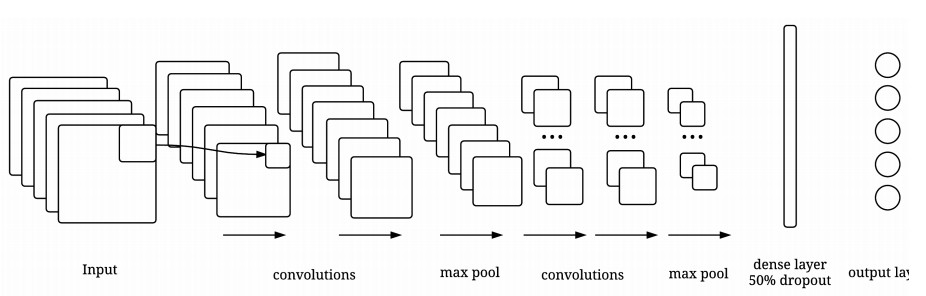
\includegraphics[scale = 0.5]{cnn_structure.jpg}
\end{figure}

\begin{thebibliography}{}
	\bibitem{1} Yakovenko, Nikolai, et al., \emph{Poker-CNN: a pattern learning strategy for making draws and bets in poker games.}, arXiv preprint arXiv:1509.06731 (2015).
\end{thebibliography}  



\end{document}  